\chapter{GETTING STARTED WITH TZUNAMI PRE-MIGRATION ANALYZER TOOL}
This chapter describes how to create an analysis report using \appName and save analyzed result for future use. This chapter contains the following topics:
\begin{itemize}
  \item Running \appName
  \item Making connection and loading ECM systems
  \item Overview of \appName window Settings for \appName
  \item Generating Report
  \item Analyzing the report generated
  \item Saving and loading, exporting the analyzed report
  \item Features of Analyzer
\end{itemize}
 \section{RUNNING TZUNAMI PRE-MIGRATION ANALYZER REPORT}

\subsection{Running \appName}
\begin{itemize}
\item To run \appName, click Start > All Programs > Tzunami > \appName - for windows 7 or older version, or
For windows 10 and above
Click    button and scroll through the alphabetical list for Tzunami. Under this locate \appName and click it to run. ECM Selection wizard appears as follows:
\begin{figure} 
  \centering
	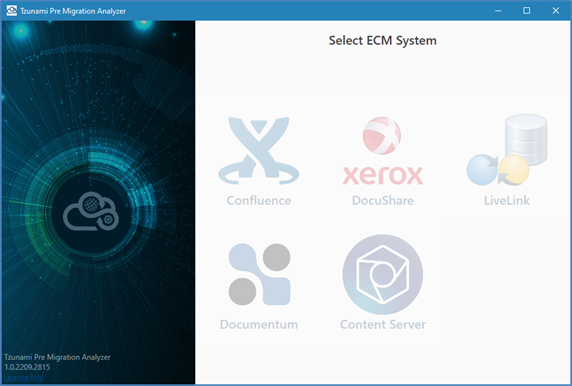
\includegraphics[width=0.8\textwidth]{Images/SelectEccmScreen.png}
 \caption{\appName, Select ECM System screen}
\end{figure}
\item Next select the required ECM system for the Analysis of the source content.
\end{itemize}
Tzunami Inc may provide the evaluation or full license based on your requirement. The evaluation license has the limitation of 10 items per folder analysis for all feature.
The \appName needs to communicate with Tzunami licensing server. Please, contact with your network administrator if there are any limitation, restriction or proxy environments and contact with Tzunami Support team. \\\\
If you cannot provide connection to Tzunami licensing server, please contact with Tzunami Support team at \href{mailto: sales@tzunami.com}{sales@tzunami.com} and inform with details. Tzunami Support team will contact back to you.
